\documentclass[aspectratio=169]{beamer}\usepackage[utf8]{inputenc}
\usepackage[english]{babel}
\usepackage{color}
\usepackage{amsmath,mathtools}
\usepackage{mathptmx}
\usepackage[11pt]{moresize}
\setbeamertemplate{navigation symbols}{}
\setbeamersize{text margin left=5mm,text margin right=5mm}
\usepackage{wrapfig}
\usepackage{bbm}
\usepackage{xcolor}
\usepackage{tabularx}
\usepackage{bm}
\usepackage{lmodern}


\newcommand{\R}{\mathbb{R}}
\newcommand{\E}{\mathbb{E}}
\newcommand{\N}{\mathbb{N}}
\newcommand{\Z}{\mathbb{Z}}
\newcommand{\V}{\mathbb{V}}
\newcommand{\Q}{\mathbb{Q}}
\newcommand{\K}{\mathbb{K}}
\newcommand{\C}{\mathbb{C}}
\newcommand{\T}{\mathbb{T}}
\newcommand{\I}{\mathbb{I}}

\setbeamertemplate{caption}[numbered]

\title{On the Uncertainty of Wind Power Generation}
\subtitle{ Waleed Alhaddad \ Raul Tempone \ Ahmad kebaier }

\begin{document}
\setbeamercolor{background canvas}{bg=blue!35}


\begin{frame}
\titlepage
\end{frame}

\begin{frame}[label=guide]\frametitle{ Introduction }
Integration of renewable resources into the urban power grid is a challenge due to uncertainties in power production. We focus on wind power. Reliable wind power production forecasting is crucial to:
\begin{itemize}
\item \textbf{Optimization of the price of electricity} for different users such as electric utilities, Transmission system operator (TSOs), Electricity Service providers (ESPs), Independent power producers (IPPs), and energy traders.
\item \textbf{Allocation of energy reserves} such as water levels in dams or oil and gas reserves.
\item \textbf{Operation scheduling} of conventional power plants.
\item \textbf{Maintenance planning} such as that of power plants components and transmission lines.
\end{itemize}

\end{frame}

\begin{frame}\frametitle{Status quo }
  Wind power forecasts can be generally categorized as follows:
  \begin{itemize}
    \item physical models
    \item statistical methods
    \item artificial intelligence methods
    \item spatial correlation methods
    \item persistence models
    \item other hybrid approaches
  \end{itemize}
 The output of such methods is usually a \textbf{deterministic forecast}. Occasionally probabilistic forecasts are produced through uncertainty propagation in the data, parameters or through forecast ensembles. However, little has been done in terms of producing \textbf{data driven probabilistic forecasts} based on real-world performance of forecasting models.
\end{frame}

\begin{frame}\frametitle{Data}
This is data from Uruguay based on \textbf{10 minute observation interval and 1000 paths}.
\begin{figure}
  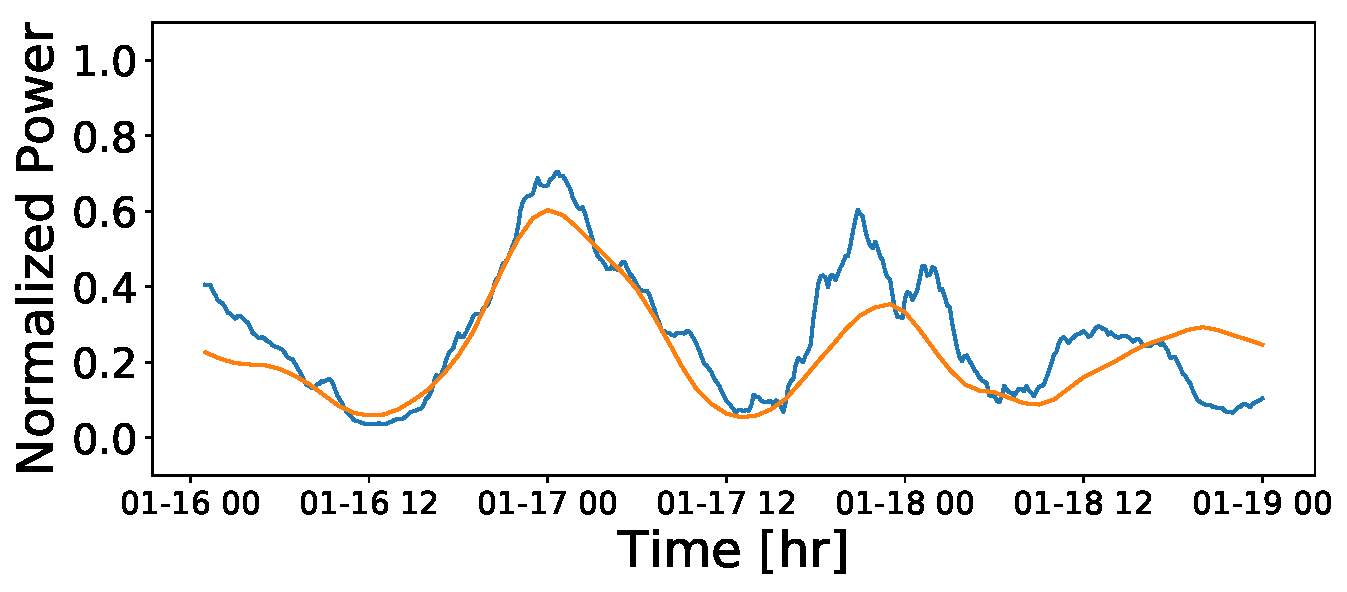
\includegraphics[width=70mm,scale=1]{plots/data_1516064400.pdf}
  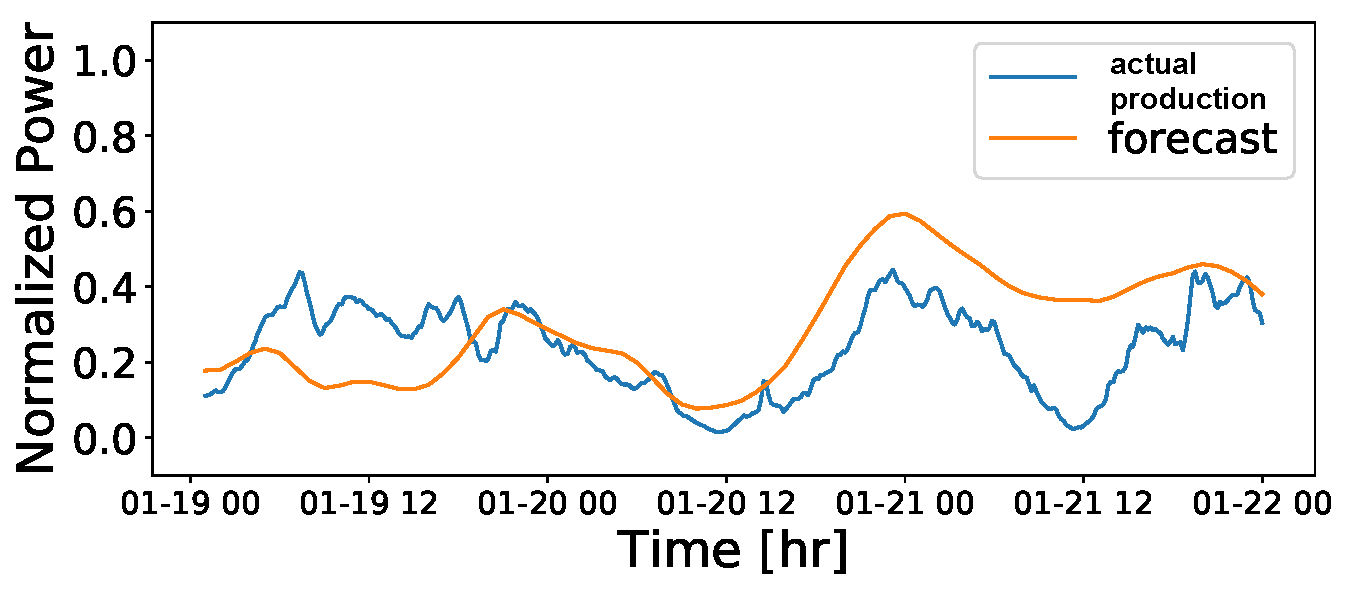
\includegraphics[width=70mm,scale=1]{plots/data_1516323600.pdf}\\
  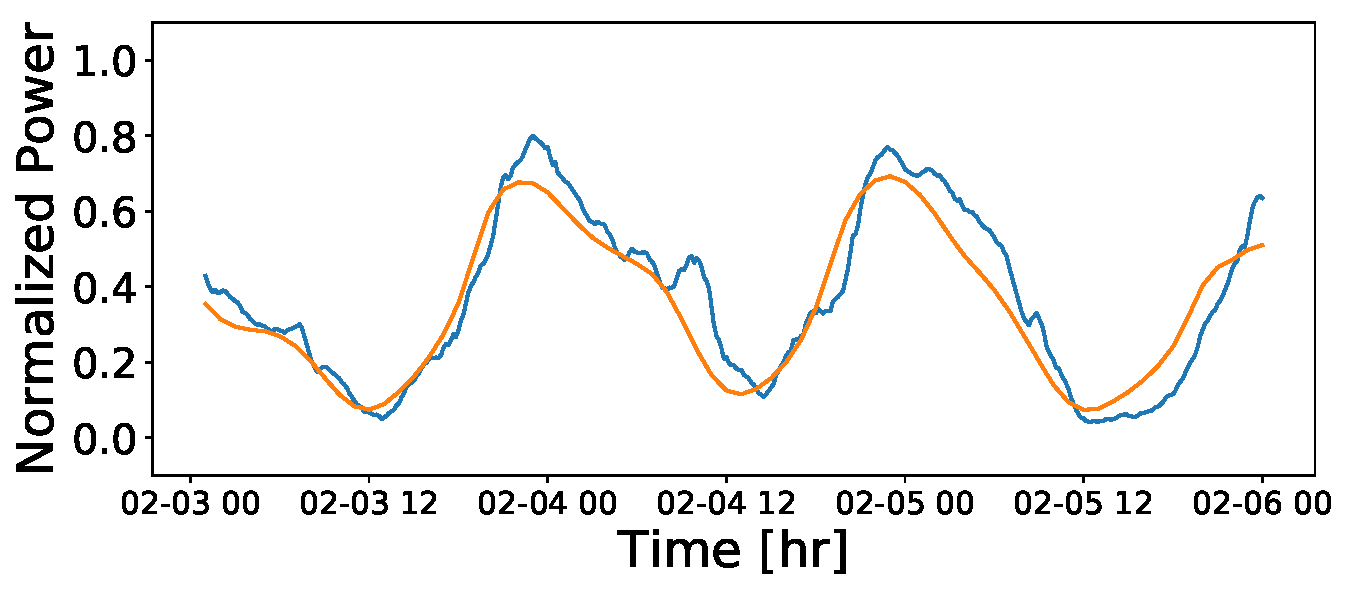
\includegraphics[width=70mm,scale=1]{plots/data_1517619600.pdf}
  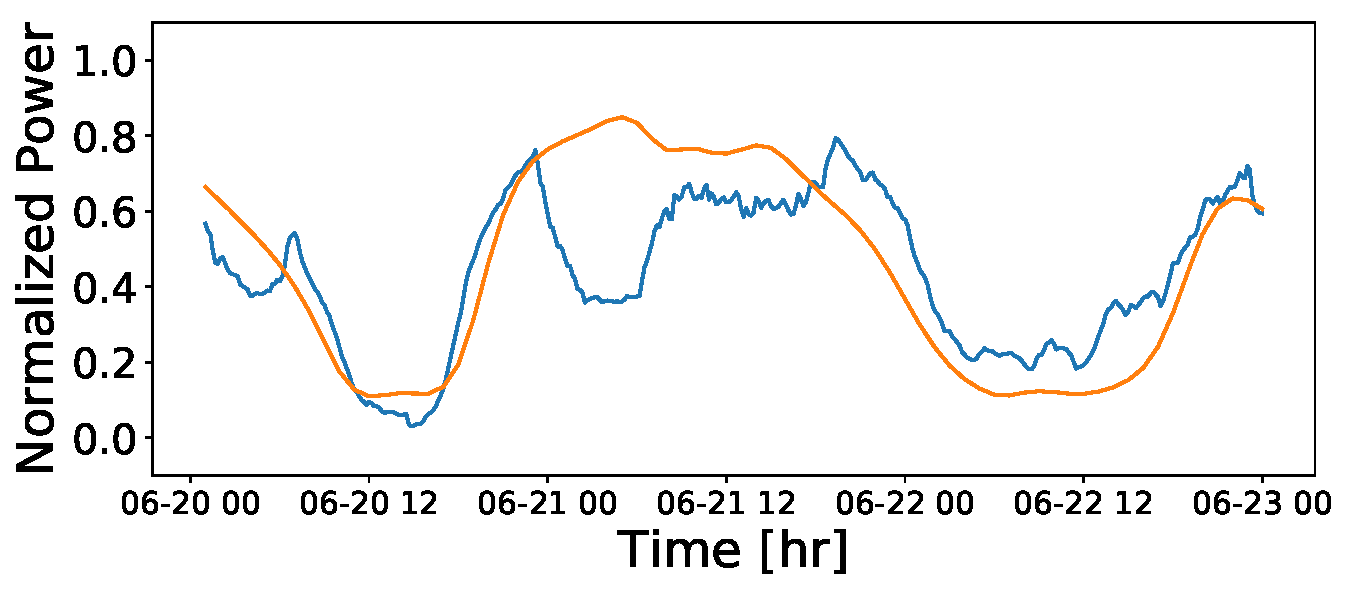
\includegraphics[width=70mm,scale=1]{plots/data_1529456400.pdf}
  % \caption{title}
\end{figure}
Have a better data set ? send it our way.
\end{frame}


\begin{frame}\frametitle{Data Skewness}
\begin{figure}
  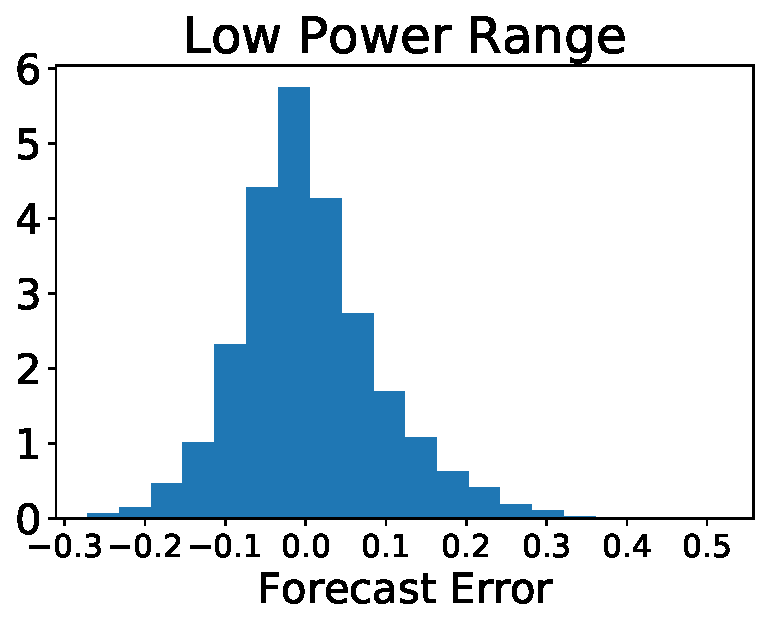
\includegraphics[width=47.5mm,scale=1]{plots/hist_low.pdf}
  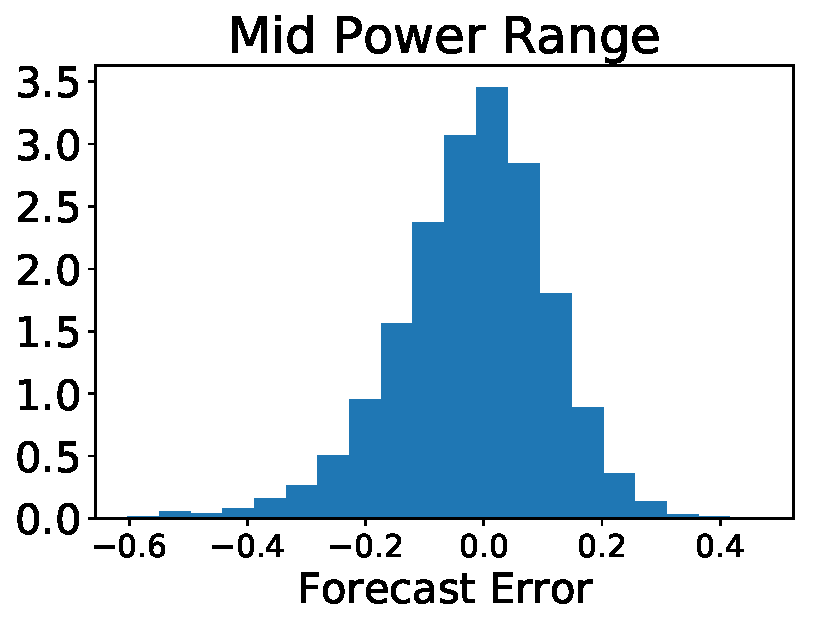
\includegraphics[width=50mm,scale=1]{plots/hist_mid.pdf}
  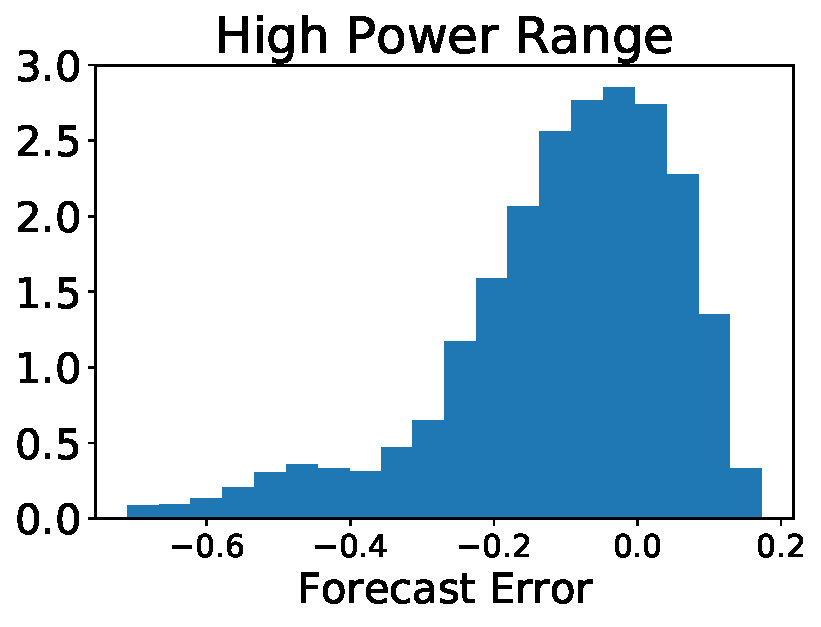
\includegraphics[width=50mm,scale=1]{plots/hist_high.pdf}
  % \caption{title}
\end{figure}
\end{frame}

\begin{frame}\frametitle{Model}
We wish to:
\begin{itemize}
  \item Generate a probabilistic forecast from a deterministic forecast.
  \item Capture the dynamics and correlation structure.
  \item Capture the skew nature of the process.
  \item Be forecasting technology agnostic. Thus, compatible with future forecasting technology.
  \item Learn from historical power production data.
\end{itemize}
\end{frame}

\begin{frame}\frametitle{Model}
We propose to model wind power\textbf{ forecasts errors using parametric stochastic differential equations (SDEs)} whose solution defines a stochastic process. This resultant stochastic process describes the time evolution dynamics of wind power forecast errors.
\begin{equation}
\begin{split}
dX_t &= a(X_t; \bm{\theta}) dt + b (X_t; \bm{\theta} ) dW_t \quad t > 0 \\
X_0 & = X_0
\end{split}
\label{main}
\end{equation}

\begin{itemize}
\item $a(\cdot; \bm{\theta}):[0,1] \to \R $  a drift function.
\item $b (\cdot; \bm{\theta} ):[0,1] \to \R$  a  diffusion function.
\item $\bm{\theta}$: a vector of parameters.
\item $W_t$: Standard Wiener random process in $\R$.
\end{itemize}

Question: How do we choose an appropriate drift and diffusion functions ?

\end{frame}


\begin{frame}\frametitle{Model}
Answer:
\begin{enumerate}
  \item We want the process to follow the wind forecast, thus we choose a drift term that is mean reverting and tracks the derivative of the deterministic forecast $p$ which is an input to our model.
  \begin{equation}
    a(X_t; \bm{\theta})=  \dot{p} \ dt - \theta_t(X_t - p_t)
  \end{equation}
where $\theta_t$ is a time-dependent paramter that controls the speed of reversion.
  \item We want a diffusion term that vanishes at the boundries to prevent the process from escaping the region $[0,1]$.
  \begin{equation}
    b (\cdot; \bm{\theta} )= \sqrt{2 \theta_t \alpha x (1-x)}
  \end{equation}
  where $\alpha$ is a constant prameter that controls the path variability.


To further ensure that the process does not escape the region $[0,1]$, the mean reversion parameter has to be selected according to the following rule,
\begin{equation}
\theta_t = \max \left( \theta_0 \ , \ \frac{|\dot{p}_t|}{\min (p_t, 1-p_t)}  \right ) \label{theta_t}
\end{equation}

\end{enumerate}
\end{frame}

\begin{frame}\frametitle{Model}
Thus, our SDE becomes
\begin{equation}
\begin{split}
dX_t&= \dot{p}_t \ dt - \theta_t(X_t - p_t) \ dt + \sqrt{2 \theta_t \alpha x (1-x)}  \ dW_t \quad t > 0 \\
X_0&=x_0\\
\theta_t &= \max \left( \theta_0 \ , \ \frac{|\dot{p}_t|}{\min (p_t, 1-p_t)}  \right )\\
\end{split}
\label{model:derivative_tracking_X}
\end{equation}
To avoid differentiation of the forecast $p_t$ and simplify, we apply a change of variables $$V_t = X_t - p_t$$ \\
The  model becomes,
\begin{equation}
\begin{split}
dV_t &=  - \theta_t V_t \  dt + \sqrt{2 \theta_t \alpha (V_t +p_t ) (1-V_t-p_t)} \  dW_t  \\ %\quad t > 0
V_0 & = v_0\\
\theta_t &= \max \left( \theta_0 \ , \ \frac{|\dot{p}_t|}{\min (p_t, 1-p_t)}  \right )\\
\end{split}\label{VtSDE}
\end{equation}
Note that this model is Markovian.
\end{frame}

\begin{frame}\frametitle{Model}
Since $V_t$ defined by the SDE in (\ref{VtSDE}) is Markovian, the likelihood function can be written as product of transition densities.

\begin{equation}
\mathcal{L}(\bm{\theta};V) =\prod\limits_{j=1}^M \prod\limits_{i=1}^N \rho ( {V_{j,i+1}|V_{j,i}}, \bm{\theta})  \rho (V_{j,0})
\label{likelihood}
\end{equation}

The transition densities can be exactly obtained by solving the following parametric Fokker-Planck equation,

\begin{equation}
\begin{split}
\frac{ \partial f }{\partial t } & (y ,t | x , s, \theta_t, \alpha )= - \frac{\partial}{ \partial y} ( a( y;\dot{p}_t , p_t, \theta_t ) f( y ,t | x , s, \theta_t , \alpha ) ) \\
& + \frac{1}{2} \frac{\partial^2}{ \partial y^2} ( b(y;\theta_t, \alpha  )  f( y ,t | x , s, \theta_t , \alpha )  ) \quad  t < s\\
\end{split}
\end{equation}
This is a parametric PDE which computationally prohibitive to solve for every transition.
\end{frame}


\begin{frame}\frametitle{Moment Matching}
Instead of solving for exact transition densities by the Fokker-Planck, we propose a \textbf{proxy transition denisty}. A suitable candidate is a Beta transition density as it can morph into symmetric and asymetric shapes.


\begin{equation}
\begin{split}
\frac{d \E[ V^k_t]}{dt} = - k \theta_t \E [ V^k_t] + \frac{k(k-1)}{2} \E [ V^{k-2}_t  b(y;\theta_t, \alpha)]
\end{split}
\end{equation}

\end{frame}



\end{document}
